\documentclass[twoside,twocolumn]{article}
\usepackage{graphicx}
\usepackage[sc]{mathpazo}
\usepackage[T1]{fontenc}
\linespread{1.05}
\usepackage{microtype}
\usepackage[english]{babel}
\usepackage[hmarginratio=1:1,top=32mm,columnsep=20pt]{geometry}
\usepackage[hang, small,labelfont=bf,up,textfont=it,up]{caption}
\usepackage{booktabs}
\usepackage{lettrine}
\usepackage{enumitem}
\setlist[itemize]{noitemsep}
\usepackage{abstract}
\renewcommand{\abstractnamefont}{\normalfont\bfseries}
\renewcommand{\abstracttextfont}{\normalfont\small\itshape}
\usepackage{titlesec}
\renewcommand\thesection{\Roman{section}}
\renewcommand\thesubsection{\roman{subsection}}
\titleformat{\section}[block]{\large\scshape\centering}{\thesection.}{1em}{}
\titleformat{\subsection}[block]{\large}{\thesubsection.}{1em}{}
\usepackage{fancyhdr}
\pagestyle{fancy}
\fancyhead{}
\fancyfoot{}
\fancyhead[C]{Ethereum 2.0 Client Metrics $\bullet$ \today}
\fancyfoot[RO,LE]{\thepage}
\usepackage{titling}
\usepackage{hyperref}
\usepackage{caption}
\usepackage{subcaption}

\setlength{\droptitle}{-4\baselineskip}
\pretitle{\begin{center}\Huge\bfseries}
\posttitle{\end{center}}
\title{Ethereum 2.0 Client Metrics 07/2020}
\author{\textsc{Afri Schoedon, \href{https://github.com/q9f}{@q9f}}}\date{\today}

\begin{document}
\maketitle
\section{Introduction}
\lettrine[nindent=0em,lines=3]{E}thereum 2.0 will be a new blockchain protocol enabling -- amongst others -- horizontal scalability through sharding and transitioning the chain to a proof-of-stake consensus algorithm.\par

\begin{figure}
   \centering
   \begin{subfigure}[t]{0.48\textwidth}
     \centering
     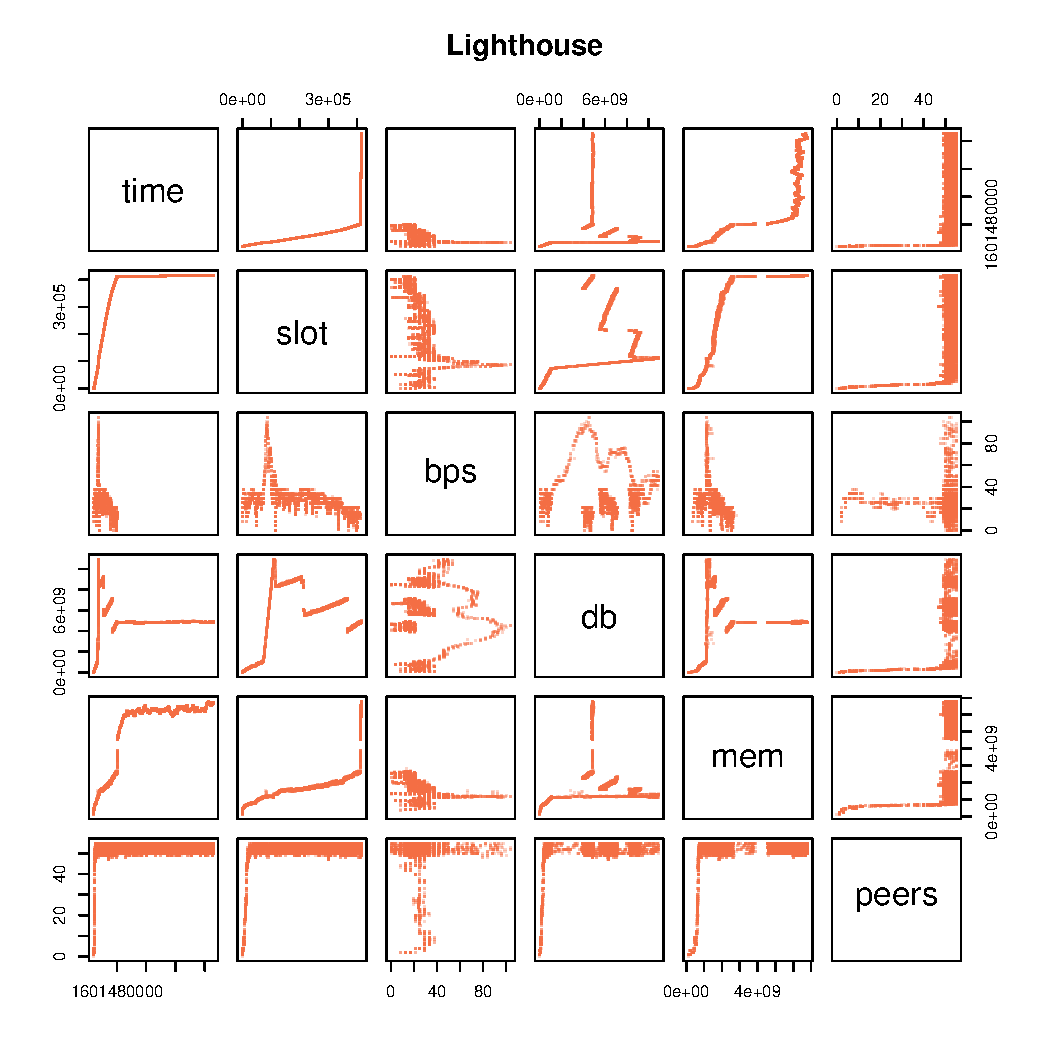
\includegraphics[draft,page=1,width=0.6\textwidth]{../res/plots.pdf}
     \caption{Lighthouse is depicted in orange.}
     \label{img:lh}
   \end{subfigure}
   \begin{subfigure}[t]{0.48\textwidth}
     \centering
     \includegraphics[draft,page=2,width=0.6\textwidth]{../res/plots.pdf}
     \caption{Prysm is depicted in purple.}
     \label{img:pr}
   \end{subfigure}
   \begin{subfigure}[t]{0.48\textwidth}
     \centering
     \includegraphics[draft,page=3,width=0.6\textwidth]{../res/plots.pdf}
     \caption{Teku is depicted in turquoise.}
     \label{img:tk}
   \end{subfigure}
   \begin{subfigure}[t]{0.48\textwidth}
     \centering
     \includegraphics[draft,page=4,width=0.6\textwidth]{../res/plots.pdf}
     \caption{Nimbus is depicted in blue.}
     \label{img:nb}
   \end{subfigure}
  \caption{All data collected is displayed in these matrices: time running, slot height, blocks per second, database size, memory usage, and peer count.}
  \label{fig:cli}
\end{figure}

\subsection{Motivation}
None of the features that Ethereum 2.0 will bring are being implemented in established Ethereum 1.x clients such as Geth or Besu. Therefore, a new generation of core clients to power the beacon chain is under development. None of these clients has ever been used in production before.\par

With the launch of the beacon chain supposedly happening in 2020, the second compilation of key metrics of four selected Ethereum 2.0 clients will be conducted, namely Lighthouse, Prysm, Teku, and Nimbus.\par

This work shall allow insights into the performance and stability of the given beacon-chain node implementations.\par

\subsection{Previous Benchmark}
In June 2020, a similar, preliminary benchmark has been conducted\footnote{\href{https://github.com/q9f/eth2-bench-2020-06}{github.com/q9f/eth2-bench-2020-06}} gathering first insights into client metrics and getting feedback from the Ethereum 2.0 core-developer community.\par

Before diving into the results, please note the following.

\begin{enumerate}
\item Most importantly, this work adds Nimbus to the list of profiled clients, allowing for a comparison of four client's metrics instead of three.
\item The numbers in this report are \textit{not} comparable with numbers in the previous report. This is mainly due to the use of different, dedicated, bare-metal hardware for determining these numbers as compared to the virtual hosts used in the previous work.
\item Unfortunately, the previous report contained a methodological inaccuracy. While all clients were run under the same conditions doing a full synchronization, the Prysm client was not built with optimized compiler settings. The team is aware and the documentation will be updated accordingly for all users\footnote{\href{https://github.com/prysmaticlabs/documentation/issues/189}{prysmaticlabs/documentation\#189}}. This has been revised and all clients are provided with release binaries.
\item Last but not least, this benchmark was conducted on the Altona testnet\footnote{\href{https://github.com/goerli/altona}{github.com/goerli/altona}}. In contrast to the Witti testnet used in the last report, the Altona testnet has a different composition of validators and currently contains fewer blocks than the Witti testnet had in June 2020.
\end{enumerate}

\subsection{Commented Data}
This article seeks to document the gathered metrics of different clients adhering to scientific methodology. It does not, however, intend to replace a peer-reviewed publication. It simply represents a version of the data commented by the author.\par

The raw data is available on Github\footnote{\href{https://github.com/q9f/eth2-bench-2020-07}{github.com/q9f/eth2-bench-2020-07}} for further analysis.

\section{Clients}
\label{sec:cli}

Four clients are used for comparing key-performance metrics.\par

\textsc{Lighthouse} is an Ethereum 2.0 client developed by Sigma Prime\footnote{\href{https://github.com/sigp/lighthouse}{github.com/sigp/lighthouse}}. It is implemented in the Rust programming language. Data referring to the Lighthouse client is depicted in orange throughout this document (figure \ref{img:lh}).\par

\textsc{Prysm} is a beacon-chain implementation written in Go\footnote{\href{https://github.com/prysmaticlabs/prysm}{github.com/prysmaticlabs/prysm}}. It is being maintained by the Prysmatic Labs team. Data referring to the Prysm client is depicted in purple throughout this document (figure \ref{img:pr}).\par

\textsc{Teku} is an enterprise-grade Ethereum 2.0 client built by the PegaSys Engineering team\footnote{\href{https://github.com/PegaSysEng/teku}{github.com/PegaSysEng/teku}}. It is implemented in Java and data referring to the Teku client is depicted in turquoise throughout this document (figure \ref{img:tk}).\par

\textsc{Nimbus} is a beacon-node implementation written in Nim built by the Status team\footnote{\href{https://github.com/status-im/nim-beacon-chain}{github.com/status-im/nim-beacon-chain}}. Data referring to the Nim-Beacon-Chain client is depicted in blue throughout this document (figure \ref{img:nb}).\par

Other clients implementing the Ethereum 2.0 protocol exist, namely ChainSafe Systems' \textsc{Lodestar}\footnote{\href{https://github.com/ChainSafe/lodestar}{github.com/ChainSafe/lodestar}}, Nethermind's \textsc{Cortex}\footnote{\href{https://github.com/NethermindEth/cortex}{github.com/NethermindEth/cortex}}, and the Ethereum Foundation's \textsc{Trinity}\footnote{\href{https://github.com/ethereum/trinity}{github.com/ethereum/trinity}}. Due to the different progress of implementing the protocol specification and core components, these clients were not considered for comparison, yet.\par

\section{Metadata}
The data is gathered on the Altona testnet. Altona is the third multi-client testnet launched with the four in section \ref{sec:cli} introduced clients as genesis validators.\par

At the time of collecting the metrics, the Altona testnet is based on \texttt{v0.12.1} of the Ethereum 2.0 beacon-chain specification. It contains approximately 120,000 slots and is run by 3,792 validators.\par

\subsection{Host Systems}
Four identical host systems have been installed for the sole purpose of the performance inspection. The host systems are dedicated bare-metal servers with an Ubuntu 20.04 LTS operating system kernel version \texttt{5.4.0-40-generic}.\par

The host machines are powered by an Intel Xeon E3-1240 v6 CPU with 8 cores. The available memory is 32 GB and the SSD disks allow for 250GB capacity.\par

\begin{figure}[t]
	\centering
	\includegraphics[draft,page=5,width=0.45\textwidth]{../res/plots.pdf}
	\caption{Synchronization progress over time.}
	\label{img:sync:prog}
\end{figure}

\begin{figure}[t]
	\centering
	\includegraphics[draft,page=9,width=0.45\textwidth]{../res/plots.pdf}
	\caption{Synchronization speed over time.}
	\label{img:sync:sped}
\end{figure}

\begin{figure}[t]
	\centering
	\includegraphics[draft,page=6,width=0.45\textwidth]{../res/plots.pdf}
	\caption{Database size over time.}
	\label{img:db}
\end{figure}

\begin{figure}[t]
	\centering
	\includegraphics[draft,page=7,width=0.45\textwidth]{../res/plots.pdf}
	\caption{Resident memory usage over time.}
	\label{img:mem}
\end{figure}

\begin{figure}[t]
	\centering
	\includegraphics[draft,page=8,width=0.45\textwidth]{../res/plots.pdf}
	\caption{Client's peer count over time.}
	\label{img:per}
\end{figure}

\subsection{Client Versions}
All clients were compiled on July 16th, 2020, from the latest available source-code targeting the version \texttt{v0.12.1} of the Ethereum 2.0 specification.

\begin{itemize}
\item \textbf{Lighthouse}: version \texttt{lighthouse/0.1.2}, compiled from \texttt{master} branch at commit \texttt{fc5e6cbb} from July 16th, 2020, with Rust version \texttt{1.44.1}-stable through Cargo.
\item \textbf{Prysm}: compiled from \texttt{master} branch at commit \texttt{df738517} from July 16th, 2020, with Go version \texttt{1.13.8} through Bazel.
\item \textbf{Teku}: version \texttt{teku/v0.12.2-dev}, compiled from \texttt{master} branch at commit \texttt{04b0a00a} from July 16th, 2020, with Java version \texttt{14.0.1} through Gradle.
\item \textbf{Nimbus}: version \texttt{beacon\_node v0.5.0}, compiled from \texttt{devel} branch at commit \texttt{3dfbc311} from July 15th, 2020, with Nim version \texttt{1.2.2} through Make.
\end{itemize}

All clients contain a built-in Altona configuration and were provided with a sufficient number of bootstrap nodes to ensure good connectivity and eliminate potential networking bottlenecks (compare section \ref{sec:perf} point \ref{sec:perf:p2p}).\par

\section{Performance}
\label{sec:perf}
This document only inspects the performance metrics of beacon-chain node implementations. Other features such as running validator clients, bootstrap nodes, or other relevant tooling are disregarded for simplicity.

\subsection{Synchronization Metrics}
Figure \ref{img:sync:prog} displays the progress of synchronizing the four aforementioned clients. Notably, the Lighthouse client manages to fully synchronize all blocks and verify all signatures in a little less than 25 minutes with the Prysm client being \textit{on par} finishing the same task in just about the same time. Teku completes the same task in 1 hour and 26 minutes, whereas Nimbus requires 6 hours and 54 minutes to fully sync and verify the Altona beacon chain.\par

Also, figure \ref{img:sync:sped} displays the same data but computing the synchronization speed in slots per second by taking the time required to fully catch up with the beacon-chain head. The plotted data points display a moving average over 60 seconds, the plotted line shows a moving average over 10 minutes. Lighthouse and Prysm lead the chart at an average of approximately 80 slots per second on the dedicated hardware.\par

The data at glance.
\begin{itemize}
\item \textbf{Lighthouse} synchronizes 122,105 slots in 1,495 seconds at an overall average speed of 81.676 slots per second.
\item \textbf{Prysm} catches up with 122,069 slots in 1,535 seconds at 79.524 slots per second.
\item \textbf{Teku} synchronizes 122,412 slots in 5,174 seconds at an average speed of 23.659 slots per second.
\item \textbf{Nimbus} catches up with 124,051 slots in 24,844 seconds at 4.9932 slots per second.
\end{itemize}

All clients do a full verification of all signatures during synchronization by default. The teams currently working on integrating new \texttt{bls} libraries which could improve these metrics even further.\par

\subsection{Database Metrics}
Figure \ref{img:db} displays the database size in Bytes plotted over time of running the nodes. The patterns are left uncommented for the client developers to analyze.\par

The data at glance.
\begin{itemize}
\item \textbf{Teku} requires 66.3 MiB after 124,342 slots.
\item \textbf{Prysm} requires 324 MiB after 124,342 slots.
\item \textbf{Lighthouse} requires 403 MiB after 124,342 slots.
\item \textbf{Nimbus} requires 3.98 GiB after 124,295 slots.
\end{itemize}

The data indicates that the Teku, Prysm, and Lighthouse clients implement database pruning by default, i.e., by removing everything that is invalidated by finalization or non-checkpointed states. The Nimbus client is running in archive mode by default.\par

\subsection{Memory Metrics}
Figure \ref{img:mem} displays resident set size reported by the four clients. Again, the patterns are left uncommented. Notably, the Nimbus and Lighthouse clients appear to be most efficient concerning memory usage, requiring around 500 MiB in default operation mode. Prysm peaks at just below 1.3 GiB.\par

Teku reports a little less than 10 GiB. The actual Java heap memory used by Teku on Altona can be assumed much lower. The off-heap memory that Java allocates is outside of the team's easy control. The JVM is being greedy about available memory, however, it is still possible to run Teku nodes on machines with very small available memory, e.g., 2GB.\par

\subsection{Networking Metrics}
\label{sec:perf:p2p}
Figure \ref{img:per} displays the peer count of every client during operation. There is not much to be commented on. This metric simply serves as a sanity check to rule out networking issues that could impact any of the other metrics.\par

Notably, there is a drastic drop in peers of the Nimbus client which, however, does not appear to correlate with any of the other metrics collected above.\par

\section{Conclusion}
The plots allow for an overview of key performance and stability metrics of the four tested clients.\par

Notably, both Lighthouse and Prysm appear to be highly optimized in their performance and mature in the implementation of the beacon-chain specification.\par

The relatively new Teku client already shows good performance but the metrics allow the conclusion that there is still room for optimization, especially regarding its memory footprint.\par

The Nimbus client which premiered as genesis validator on the Altona testnet shows potential for implementing further features such as pruning and optimizations of the networking and verification code.\par

\vspace{\fill}

\section*{Note}
The author is not affiliated with any of the teams implementing an Ethereum 2.0 client. The author is independently funded through the Ethereum Foundation's Ecosystem Support Program\footnote{\href{https://esp.ethereum.foundation}{esp.ethereum.foundation}} and the Goerli Testnet Initiative\footnote{\href{https://goerli.net}{goerli.net}}.\par

The author is not speaking on behalf of any organization.\par

A warm note of thanks goes out to everyone who reviewed the initial June-2020 report and provided valuable feedback allowing for a more accurate data gathering in this subsequent report.\par

And finally, a big thanks to the client teams patiently answering questions and sharing insights about the protocol implementations.

\texttt{:)}
\end{document}
